%%%%%%%%%%%%%%%%%%%%%%%%%%%%%%%%%%%%%%%%%%%%%%%%%%%%%%%%%%%%%%%%%%%%%%%%%%%%%%%%%%%%%
% Machine Learning in Prediction
%
% 1. Linear Models
% 2. Polynomial Models
% 3. Neural Networks
% 4. Linear parameter-varying models
% 5. Adaptive nature using ISIS algorithm
% 
%%%%%%%%%%%%%%%%%%%%%%%%%%%%%%%%%%%%%%%%%%%%%%%%%%%%%%%%%%%%%%%%%%%%%%%%%%%%%%%%%%%

Cheap data storage and escalation of computational power allowed the world to enter a new age: the age of \textit{big data}. With vast amounts of data, previously in-viable and data hungry machine learning algorithms are now implementable.  The technology sector was the first group to be able to exploit this arcane technology to create tremendous value in applications ranging from targeted advertisements to self driving cars. The value was so great that the current top four companies in America by market capitalization are all technology companies (Microsoft, Apple, Amazon, and Facebook) as of 2019. As the technology sector's successes grow, other industries begin to catch a glimpse of the potential value creation in their own respective industries and initiate their own digital revolution. The ripples of success from the technology industry ultimately resulted in waves of capital investments into machine learning (ML) and artificial intelligence (AI) from all industries.

ML solutions promise to be cheaper, more accurate, and have online learning abilities compared to traditional methods.  Additionally, the solutions are promised to be easier to implement and will take less time to design; feed it data and it will learn, as they claim.  With this mentality, machine learning engineers and data scientists from technology companies attempted to conquer other industries, one industry being process control and chemical engineering. Unfortunately, their crusade fell short and their successes were few due to their lack of engineering knowledge and inability to identify large value gains.  Typically, projects in technology companies deal with very unambiguous information such as identifying location of objects or predicting the enjoyments of an individual based on previous articles they have read. However, process control typically generate time-series data and are often very ambiguous with data characteristics unique to the industry. Some characteristics include time delayed data, multi-modal data, unreliable data, highly noisy data, state transition dynamics data, and any combination of the prior.  Due to the increased complexity, data pre-processing for ML projects in the process control industry is mission critical and much more vigorous to ensure successful applications.

Table \ref{tab:2MLApplications} shows some general machine learning applications for the process control industry. Currently, ML applications in the process industry can be broken down into prediction, monitoring, and control.  The field of prediction deals with mapping from certain inputs to desired outputs. An example would be building a soft sensor to predict for a state, $x_{m}$, that is expensive to measure.  By identifying states highly correlated to $x_{m}$, a multivariate soft sensor can be built to inexpensively predict the state in the future. In ML monitoring, the algorithms are tasked to monitor the process for anomalous activities. Here, an example would be applying a classification method to predict for failures in process equipment.  Lastly, ML control is concerned with the topics of adaptive, multivariate optimal control. Reinforcement learning is the typical ML algorithm for control.  

\begin{table}[h]
    \centering
    {\setstretch{1.2}
    \begin{tabular}{c|c|c}
    Prediction & Monitoring & Control \\ \hline
    Soft sensing & Anomaly detection & Supervisory control \\
    Forecasting  & Anomaly prediction & Regulatory control \\
    Operator education  & Alarm prioritization & Operator education \\
    Digital twin  & Alarm reduction & Multivariate control\\
    \end{tabular}}
    \caption{General applications for machine learning in the process control industry.}
    \label{tab:2MLApplications}
\end{table}

 Figure \ref{fig:02AICloud} shows a the machine learning architecture that is generic enough for implementation in all industrial plants. First, the industrial process (e.g. refinery, pipeline, reactor, etc.) sends raw sensor data into the cloud, where it is cleansed through data pre-processing methods.  Then, the filtered data is sent into different machine learning algorithms depending on the objective of the application and will output the desired values.  After a set time frame, all ML models will then be re-updated to learn the newest experiences. For computations requiring speedy outputs, portions of the ML code can also be pushed to the local devices using Microsoft Azure IoT edge devices. 

\begin{figure}[h]
    \centering
    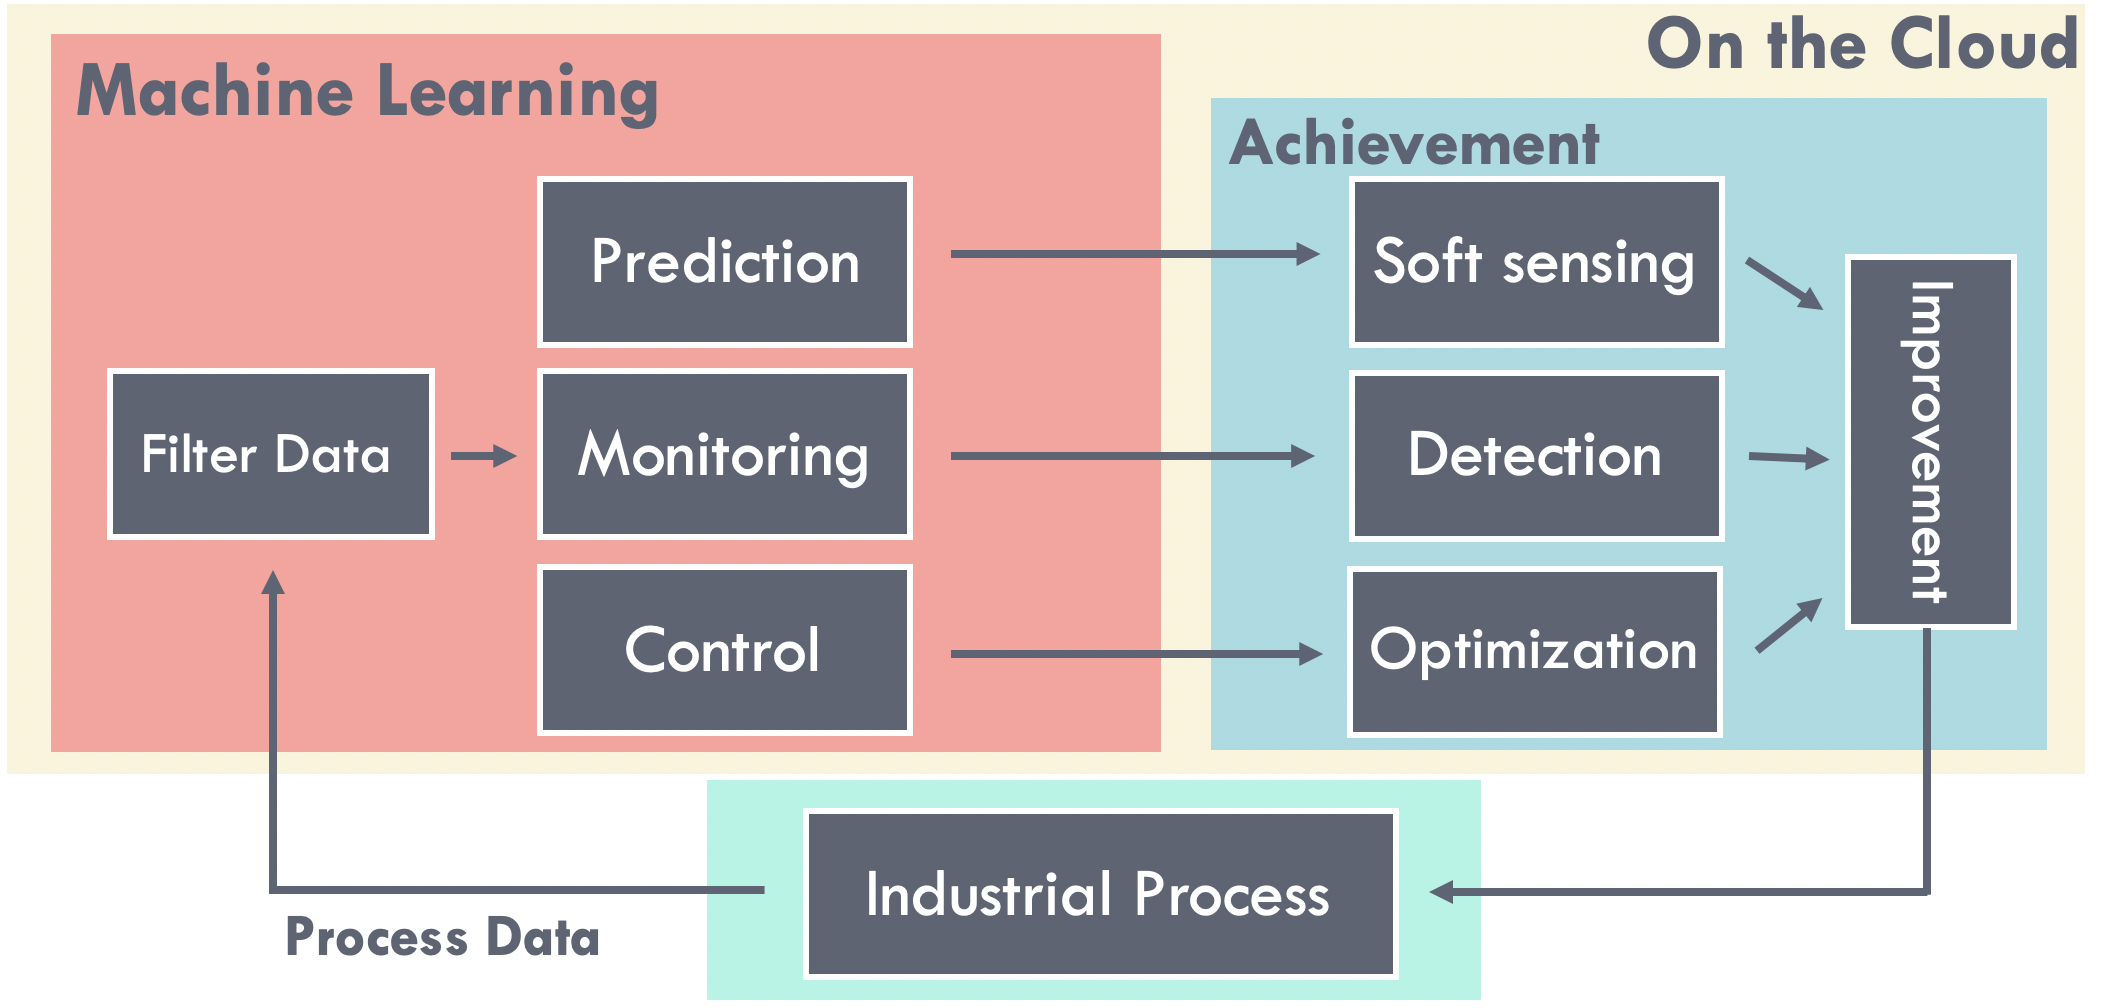
\includegraphics[width=\textwidth]{images/ch2/02AICloud.png}
    \caption{Overall machine learning architecture in an industrial environment}
    \label{fig:02AICloud}
\end{figure}

The objective of this chapter was to convey ideas for implementing machine learning solutions catered towards the \textbf{process control} industry.  In this chapter, the first half consists of common data pre-processing techniques to handle common process control concerns and is visually described by the "Filter Data" box.  The second half contains machine learning methods (in order of difficulty) to handle different process control prediction problems ("Prediction" box in the above figure). For validation, the machine learning methods were implemented live onto an industrial pipeline for prediction, monitoring, and optimization\footnote{This project was supported in part by Mitacs through the Mitacs Accelerate program and the algorithms went live as of May 7th, 2019.}\footnote{This chapter only contains the theory, application, and highlights. The detailed industrial project report can be found in Appendix A.}.

\section{Data Pre-processing}
Data pre-processing typically includes many steps starting with filtering by subject matter expertise, and then transitioning to common statistical methods.  For this section, only the filtering methods unique to process control will be discussed. Please refer to Appendix A for details regarding the other steps. Process control is typically concerned with multivariate time-series data plagued with noisy and/or unreliable sensor readings. Time delays are critical to successful prediction applications in process control. Furthermore, some processes may also have a variety of different operating regimes depending on downstream demand or ambient conditions.  In order to have successful prediction algorithms for process control, all of the above must be considered.

\subsection{Time Delay Data}
Time delay is the time between the performance of a control action and the change in output. Time delays occur due to the physics of the natural world.  For example, turning on a pump at the beginning of a pipeline does not result in higher flow rates immediately.  The process takes time to adjust and \textbf{transition} to the new steady state; therefore, raw data must be first shifted to account for the time delay.  Without doing so, models would be using current information to predict the past.  Imagine building a model to predict for the outlet flow rate of a pipeline where the regressors are pump statuses 300 km upstream of the outlet.  If a change in pump status occurred at $t = 0$, the pressure will take a few minutes to propagate down the pipeline.  Thus, the model taking pump statuses at $t = 0$ must have its flow rate labels shifted from $t = \tau$, where $\tau$ is the expected time delay.  An example of the time delay shifting procedure for an industrial pipeline is shown in Table \ref{tab:08TimeToCC} located in Appendix A, where data was shifted for different locations along the pipeline to enhance predictive capabilities.

Initial engineering expertise and/or data analysis must be conducted to identify the time delay for specific processes.  For example, it is well known that pressure propagates down incompressible fluids at approximately the speed of sound (1480 km/h) \cite{fluid_mechanics}.  Using this information, adjusting for the time delays along the pipeline was made trivial.

\subsection{Multi-modal Data}
In the process industry, it is common to have multiple modes of operation due to changing ambient conditions (e.g. summer, winter), different market demands, and a variety of other factors.  Each operating condition also consists of unique equipment operation and process characteristics (flow rates, temperatures, etc.); therefore, a common model to predict for many different operating conditions lead to increased model errors.  Here, unsupervised learning should be used to avoid this scenario for systems with many modes.  More specifically, clustering methods should be applied to segregate data from different operating modes, and separate models should be built using data from each operating mode to enhance accuracy.  For big data applications, \textit{k}-means or density based scanning (DBSCAN) should be used due to their scalability and non-iterative nature \cite{clustering_complexity}. Of the two methods, \textit{k}-means is much faster while DBSCAN is more robust to outliers.

An example of the breakdown of a multi-modal system can be found in Figure \ref{fig:08DBSCAN} in Appendix A.  By segregating the system into multiple modes, more accurate weights can be identified for each mode compared to general weights for all modes.  In fact, most modes would not even use the same equipment.  Such a concept is similar to using a linear parameter-varying model to approximate a non-linear system.  

\subsection{Unreliable and Noisy Data}
Thousands of measured data are recorded per minute on modern distributed control systems. However, many process variables such as viscosity, or parts per million (ppm) are difficult to measure with modern equipment on a live process. This results in inaccurate values being sent to the ML models, ultimately reducing accuracy.  To overcome highly unreliable data, a general strategy is to identify how the operator(s) are using the data and to engineer the feature(s) to be used in the same way for the ML model.  For example, the densitometers installed along the industrial pipeline shown in Appendix A all show different readings for the same crude. At times, the reading could be off by $\pm 20\%$. However, the operators only use the density reading to determine the grade of crude inside the batching pipeline. The crude is light if the API is above a threshold, heavy otherwise.  The physical number had no meaning for them.  To improve the ML model accuracy, the density reading was feature engineered to be a binary variable reading "1" if the API was above the threshold, "0" otherwise.  By doing so, the variable in the ML model was used in the same way as the operators and the accuracy increased.

Other data measurements may be accurate, but highly noisy. Noisy measurements may lead to significant predictive errors 
Noise can be reduced significantly by applying an exponentially weighted moving average (EWMA) filter given by:
\begin{equation}
    v_t = \beta v_{t - 1} + (1 - \beta) \theta_t, \; v_0 = 0
    \label{eq:08EWMA}
\end{equation}
\begin{equation}
    v_t \leftarrow \frac{v_t}{1 - \beta^t}, \forall v \in V
    \label{eq:08Bias_Correction}
\end{equation}
where $v_{t}$ is the exponentially weighted value at time $t$.  $\beta$ is the exponentially weighing factor.  Larger $\beta$ results in smoother results.  $\theta_t$ is the original value at time $t$. $V$ is a vector representing the exponentially weighted values before bias correction. EWMA is a very effective way to remove noise in chemical processes because these processes typically contain slow dynamics. By exponentially smoothing the data, the fast peaks are removed while preserving the slow dynamics. An example of the EWMA algorithm applied to the measurement of drag reducing agent (DRA) ppm values is shown in Figure \ref{fig:08DRA} in Appendix A.  DRA ppm measurements are known to be highly noisy; however, the noise can be almost completely removed by applying EWMA.

\subsection{State Transition Dynamics}
Another unique topic of process control is the dynamics of the system. System dynamics refer to the transitional period of going from one steady state to another after a control input is provided. Typically, dynamical models are used for advanced process controls where optimizing for the dynamics of the system is critical for optimal performance.  In order to build machine learning models to describe the dynamics of systems, a time-series implementation must be pursued.  Typical ML models map states and control actions at time $t$ to the desired output at time $t_{ss}$, where $t_{ss}$ is the time required for the system to transition to the new steady state.  By doing so, the dynamics of the system are completely omitted.  In order to build a dynamical ML model, the raw data needs to skip the time delay pre-processing step and be augmented by time.  Imagine a simple single-input single-output (SISO) system:
\begin{equation}
    y = w_1x + b
\end{equation}
In time-series implementation, the model would instead be:
\begin{equation}
    y_{t + 1} = w_1x_{t} + w_2x_{t - 1} + w_3x_{t - 2} + ... + y_{t} + y_{t - 1} + ... + b
    \label{eq:02_1step}
\end{equation}
where the input vector would be augmented as $\mathcal{X} = [x_{t} | x_{t - 1} | x_{t - 2} | ... ]$. Here, Equation \ref{eq:02_1step} becomes the 1-step ahead predictor of the system and dynamics can be predicted for. This data augmentation method is identical to all ML models if a time-series implementation is desired. In Appendix A, Figure \ref{fig:08ts_ls} shows an example of a time-series prediction model.  Because such models only predict one step in advance, error is typically very low.  The predicted value can also be fed in recursively to generate a infinite step ahead prediction that can be used for forecasting long term trends.

\section{Machine Learning Methods}

Many ML methods exist for prediction, each having its advantages and disadvantages. In this section, the most common ML methods will be shown along with their applications in process control.  Unique hyper parameters for different ML methods will also be shown; however, common hyper parameters such as $\alpha$, training epoch, and mini-batch size are common throughout and will be omitted.

\subsection{Linear Models}
Linear models have two variants, linear regression and logistic regression.  The former is used for prediction tasks associated with continuous variables while the latter is used for classification tasks.  For example, linear regression is a great algorithm for soft sensor applications whereas logistic regression is more suitable for monitoring for anomalous activities. In this chapter, only the prediction variant will be shown. The model structure of linear regression is given as:
\begin{equation}
    \hat{y} = W_1^Tx + W_2^Tu + b
    \label{eq:02LS}
\end{equation}
where $x \in R^n$ is a vector of states, $u \in R^{m}$ is a vector of inputs and superscript $T$ denotes the transpose operation.  $\hat{y}$ is the predicted variable and can be anything; in soft sensors, $\hat{y}$ would be the "soft sensed" variable.  

The most common model structure for ML in the process control industry are linear models despite all processes being non-linear.  This is because the narrow region most processes operate around can typically be assumed to be linear \cite{process_control_ref13}.  Additionally, linear models are simple, interpretable, and require low amounts of data. However, the draw backs of linear models are their poor performance in the big data era where large amounts of data is available (see Figure \ref{fig:02learning_aggro}).  This trait is intensified given high dimensional data sets where identifying interaction effects are critical for accurate predictions.

Linear models were applied to the industrial pipeline as a benchmark algorithm.  The performance of the linear models can be seen in Tables \ref{tab:08LSperformance}, \ref{tab:08ConstLSPerformance} and Figures \ref{fig:08LSPlots}, and \ref{fig:08CLSPlots}. 

\begin{figure}
    \centering
    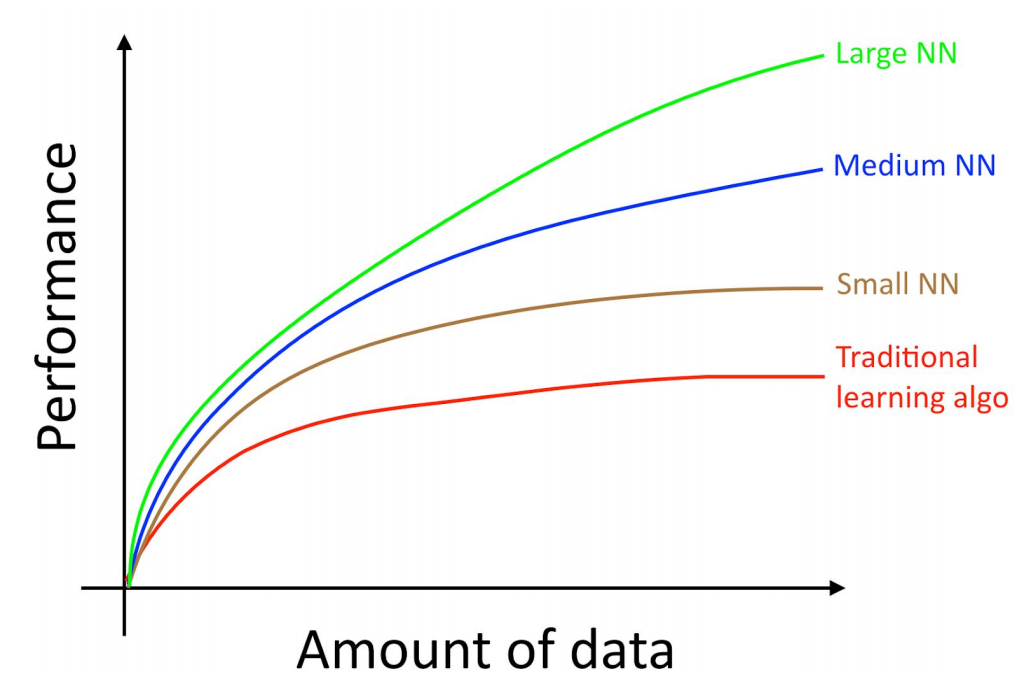
\includegraphics[width=0.7\textwidth]{images/ch2/02Learning_Aggro.png}
    \caption{Performance as a function of data.  Original image from \cite{deeplearning_course}.}
    \label{fig:02learning_aggro}
\end{figure}

\subsection{Polynomial Models}
Polynomial models are a general class of non-linear models that explores the main and interaction effects of its regressors.  The general model structure of a two regressor polynomial model is given by:
\begin{equation}
    \hat{y} = w_1x_1 + w_2x_2 + w_3x_1^2 + w_4x_2^2 + w_5x_1x_2 + e
\end{equation}
where $w$ are the weights, $x$ are the regressors, and $e$ is the modelling error.  In this model, linear, quadratic, and interaction effects are all explored simultaneously. However, the amount of parameterization required for a high dimensional prediction problem using this model structure might be difficult to interpret, thus, a truncated version of the model could be used instead for high dimensional problems. One special case of a truncated polynomial model is the exponential model given by:
\begin{equation}
    \hat{y} = w_1 x_1^{w_2} + b
\end{equation}
where the power of the regressor is also a weight to be identified. This is advantageous in situations where the non-linearity of the system is unknown. A quadratic and square root version of the exponential model were applied to the pipeline and the performances are shown in Table \ref{tab:08quad_sqrt_performance} and Figure \ref{fig:08PolynomialPlots}.  Compared to the linear models, the errors were reduced by up to 10\%.

\subsection{Neural Network and Deep Learning Approaches}
Neural network and deep learning approaches shine for predictive tasks where predictive power is the primary driver, while interpretability is not an issue, and acceptable\footnote{Neural network models are typically executed on servers and the outputs are sent to the actuators.  For fast processes, deep learning models should be pushed to the edge device.} hardware exists.  Deep learning is a special case of neural networks where many hidden layers exist.  The general consensus of the AI and ML community is that any neural network with more than three hidden layer is considered deep learning; however, the idea is not concrete and is open to personal preference.  The neural network model structure is highly non-linear and attempts to explore interaction effects of all regressors.  For a more detailed explanation on neural networks, the notation of its the variables, and its theory, please refer back to Chapter 1. Only a brief summary of the theory will be provided here. Due to the model complexity and high parameterization of neural networks, its predictive powers are unparalleled compared to other methods and can fit any function. In \cite{nn_fit}, the authors showed that:
\begin{framed}
\begin{quote}
There exists a two-layered neural network with ReLU activation functions and $2n+d$ weights that can represent any function on a sample of size $n$ in $d$ dimensions. 
\end{quote}
\end{framed}
Three distinct types of neural networks exist: i) Multilayer perceptrons (MLPs); ii) Recurrent neural networks (RNNs); iii) Convolutional neural networks (CNNs).

A visual representation of a MLP is shown in Figure \ref{fig:02MLP}.  MLPs (also known as feedforward neural networks) are the simplest and most common of the three.  In MLPs, the outputs of each neuron, $a_j^{[r]}$, is computed as:
\begin{equation}
    a_j^{[r]} = f(w_1x_1 + w_2x_2 + ... + w_mx_m + b)
\end{equation}
where the function, $f$, is non-linear and known as the \textit{activation function}.  The purpose of $f$ is to introduce non-linearity to the model; a critical addition because no process in the real world is linear.  In an intuitive sense, MLPs can be visualized as a brute force approach to identify the interaction effects of every regressor with each other. Due to the sheer number of parameterization, MLPs are very effective in predicting in-sample data points.  However, the models suffer tremendously during events where the testing data is significant different.  Large MLPs also tend to overfit; thus, it is critical to increase regularization as the MLP increases in size.

\begin{figure}[h]
    \centering
    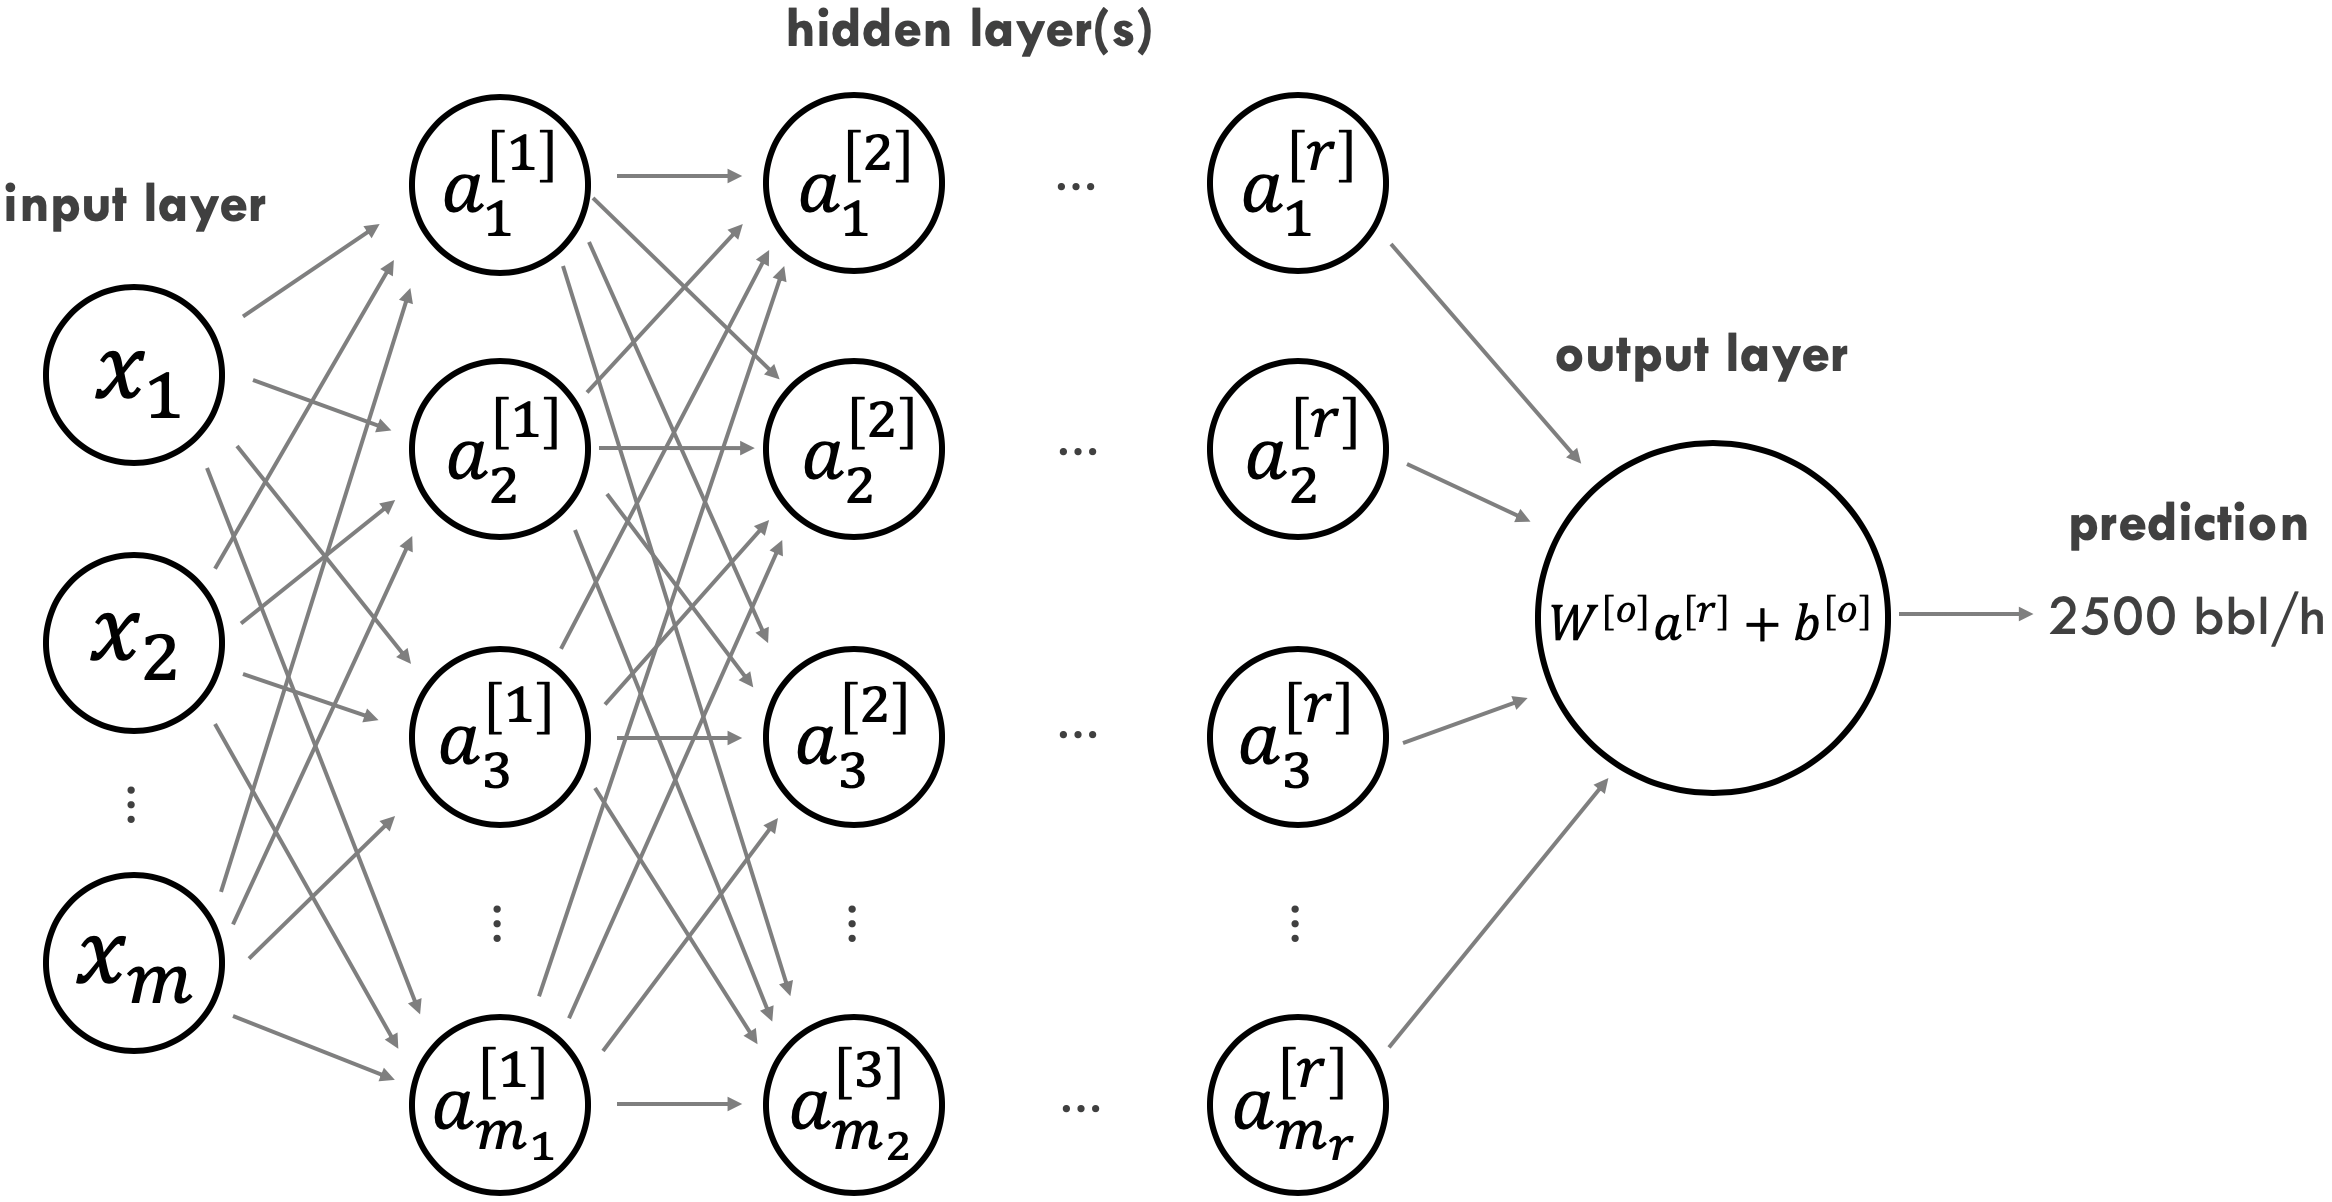
\includegraphics[width=0.9\textwidth]{images/suncor/08NN.png}
    \caption{Structure of a general neural network.}
    \label{fig:02MLP}
\end{figure}

MLPs were also applied to the industrial pipeline to model for the outlet flow rate. The input variables were measurements of variables along the pipeline such as temperatures and pressure, and the output was the outlet flow rate. Three different MLPs with varying sizes were applied.  Their respective performances can be seen in Table \ref{tab:08_nn} and Figure \ref{fig:08PolynomialPlots}.  It can be seen that the performance on the training and validation data were both excellent, though the error on the testing data increased significantly.  This was caused by the testing data being significantly different from the training data.  Data for model training was collected during the winter months, but was tested on summer months where the temperatures increased by up to $\ang{10}$ C. The increase in temperature resulted in reduced viscosity of the shipped crude and significantly hindered the predictive power of the MLPs. Ultimately, the MLPs' performance on the test data was almost identical to the much simpler polynomial models and was not used.

An especially useful type of neural networks for the process industry are RNNs (Figure \ref{fig:02RNN}) due to their time-series architecture.  Naturally, RNNs are set up to be infinite step ahead predictors and identifies temporal correlations within the data.  Traditional applications of RNNs can be found in speech recognition, translation, and language modelling.  In the process control industry where time-series data is abundant, RNN is the natural choice for typical soft sensing applications.  On a high level, RNNs accept inputs $x_t$, and outputs $y_t$.  At the same time, $y_t$ is sent as an input, along with $x_{t+1}$, back into the RNN to compute for $y_{t+1}$.  A similar computation is conducted until the end of the sequence of inputs.  By recursively re-inputting outputs as input data, RNNs are able to predict for an output trajectory given an input trajectory.

\begin{figure}[h]
    \centering
    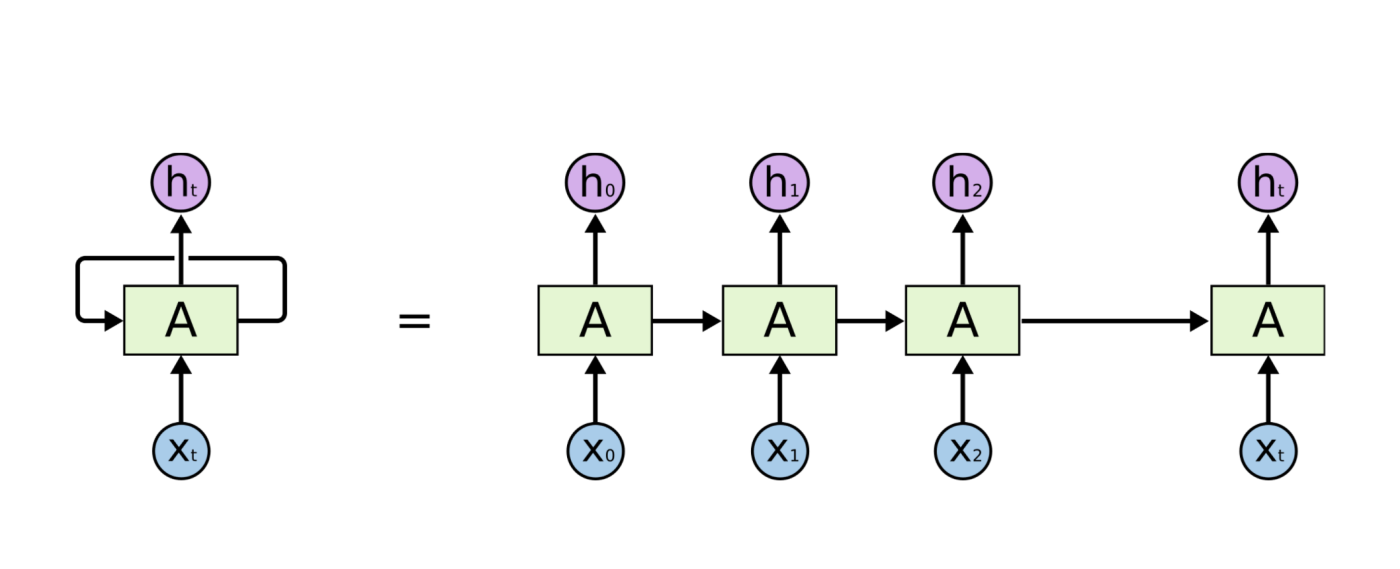
\includegraphics[width=0.9\textwidth]{images/ch2/02RNN.png}
    \caption{Architecture of a RNN.  Original image from \cite{NN}}
    \label{fig:02RNN}
\end{figure}

CNNs are the last type of neural networks and are typically used for computer vision applications. The architecture of a typical CNN can be found in Figure \ref{fig:02CNN}. Unlike its predecessors, CNNs make the explicit assumption that inputs to the network will be images. This enables certain properties to be encoded into the architecture, making the forward pass more efficient while reducing the number of parameters.  More specifically, CNNs assume all inputs are arranged in three dimensions: height, width, and depth.  The height and width are simply the resolution of an image while the depth is the amount of color channels.  For example, a coloured image contains 3 channels (red, green, blue) while a grayscale image contains only one.  From this assumption, the weights of CNNs only need to be applied to specific locations, without the need of fully connected layers.  Furthermore, the input data will then be downsampled using pooling layers to extract the most important features while discarding the rest.  

\begin{figure}[h]
    \centering
    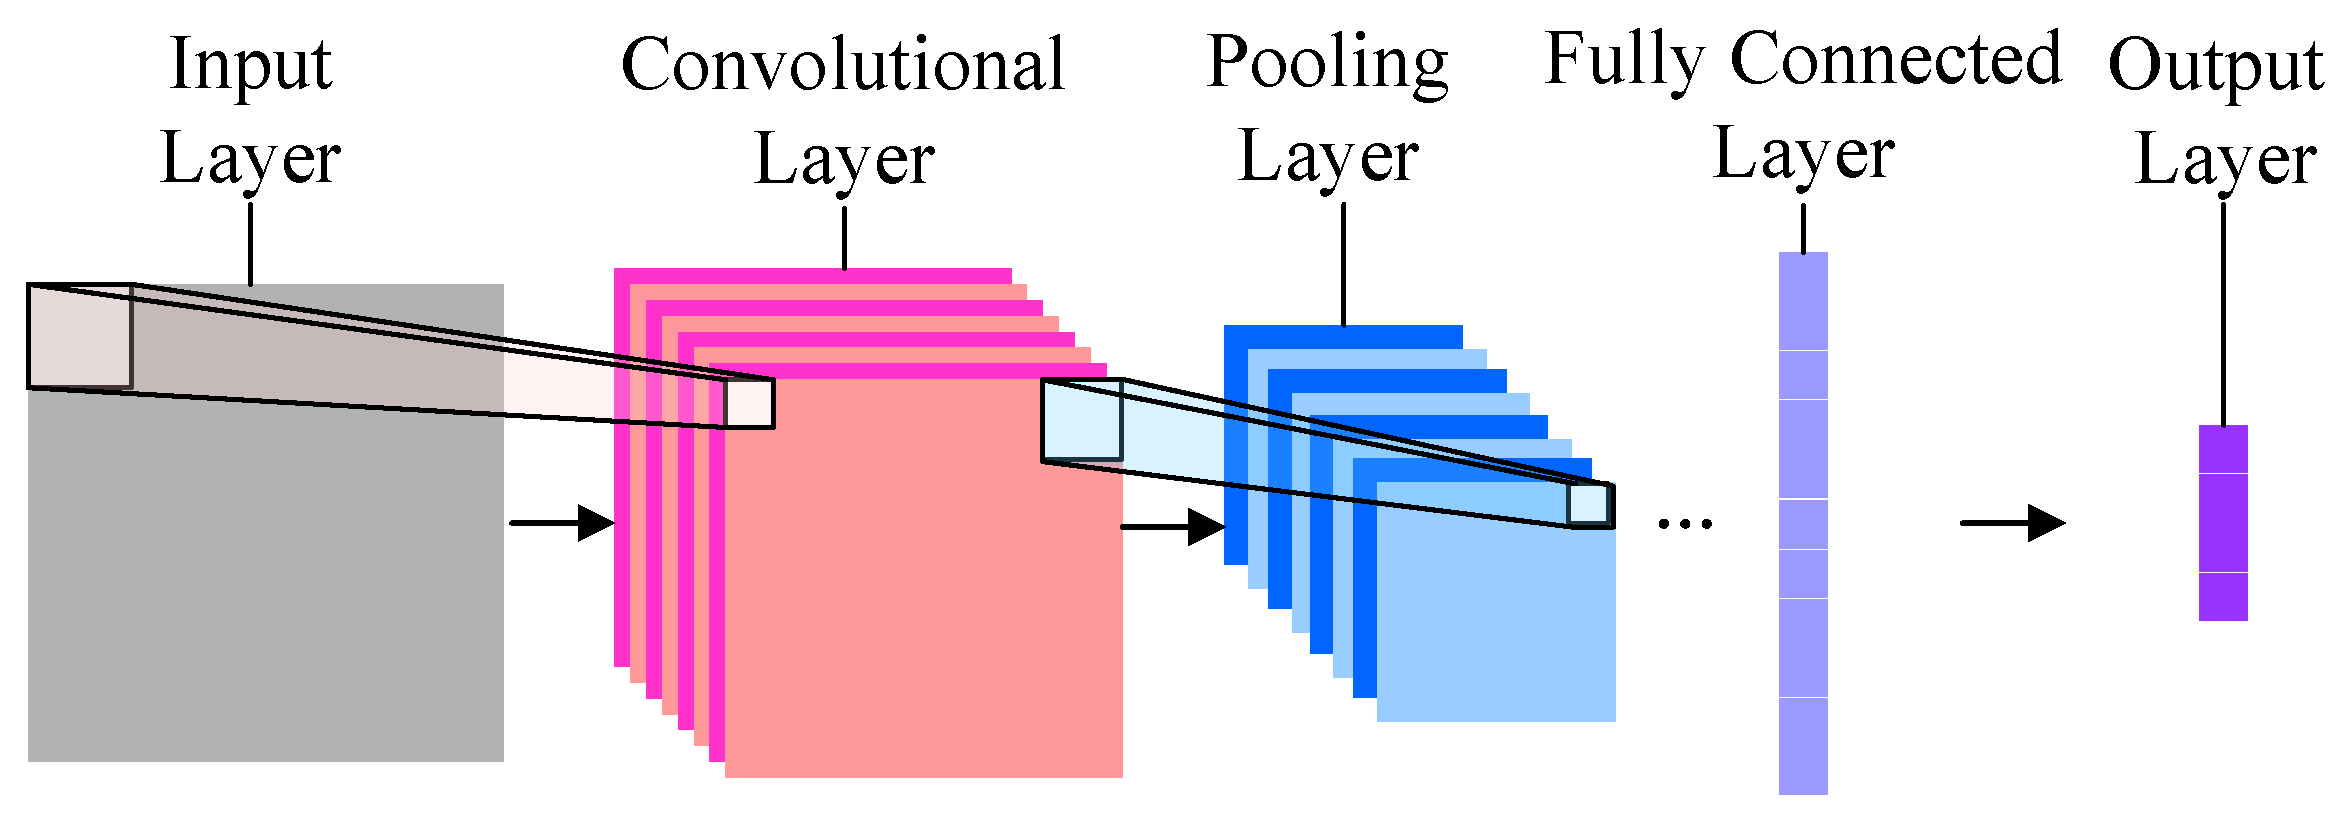
\includegraphics[width=0.9\textwidth]{images/ch2/02CNN.png}
    \caption{Architecture of a CNN.  Original image from \cite{NN}}
    \label{fig:02CNN}
\end{figure}

In the process industry, CNNs can be leveraged as a soft sensor to measure variables using cameras. An example would be detecting the level of crude inside a primary separation vessel using the sight glasses, since traditional methods are not as effective.

Both CNNs and RNNs were not applied to the industrial project directly, but were provided to the reader as \textbf{advanced} methods for future projects that command exceptionally high predictive power, or computer vision soft sensing capabilities.  More information regarding RNNs and CNNs can be found in \cite{NN}.

\subsection{Linear Parameter-varying Models}
Linear parameter-varying models (LPV) are last type of ML models that were applied to the industrial pipeline.  

\subsection{Adaptive Modelling: Importance Sampling Incremental Learning (ISIS)}

